
\section{Experimenting with object affordances}

\label{sect:experiment}

\ifverbose
The latest instantiation of the ``general principle'' we would like to
dwell upon is related to mirror neurons. It turns out that the causal
chain here is more complicated. This requires a more complicated
structure to support it.
\fi

Poking moves us one step outwards on a causal chain away from the
robot and into the world, and gives a simple experimental procedure
for segmenting objects.  There are many possible elaborations of this
method, all of which lead to a vision system that is tuned to 
acquiring data about an object by seeing it manipulated by the robot.  

This kind of active segmentation will nevertheless be inconvenient in many situations if not 
coupled with a mechanism to learn from experience. For example, it 
would be terribly inefficient to always have to poke an object first
before it could be grasped.
It would be much better if the robot could learn about
objects and, in particular, how to identify a previously encountered object. 
A further difficulty, at least for a robot with a simple 
manipulator (such as Cog's flipper), is that ``affordances'' are scarce: 
most of the time the object will simply move from one position
to another if we are willing to discount when it falls from the table.

However, for objects that roll there is a cue the robot can exploit
to understand their behavior. An object that rolls tends to do so even 
if it is not poked precisely. We selected a small set of objects to
experiment with: a cube, a toy car, an orange juice bottle, and a ball.
Affordances are not only a property of the mechanics of the object, but 
rather a combination of visual appearance, of the object's physical 
composition, and of the ability of the actor. We selected a measure of
the principal axis of the object (easily obtained from the segmentation)
as a visual component of the affordance. Table \ref{tab:affordances} 
shows the expected behavior.

\begin{table*}[htbp]
\begin{center}
\begin{tabular}{|p{2cm}|p{3.5cm}|p{5cm}|}
\hline
{\it object} & {\it angle between principal axis and preferred direction of rolling} &  {\it behavior} \\ \hline\hline
{\bf cube} & n.a. & no principal axis, does not roll\\ \hline
{\bf car} & $0^\circ$ & rolls along the principal axis\\ \hline
{\bf bottle} &  $90^\circ$ & rolls at right angle\\ \hline
{\bf ball} &  n.a. & no principal axis, does roll\\ \hline
\end{tabular}
\caption{
%
Behavior of a small set of objects when poked at random by the robot manipulator.
%
}
\label{tab:affordances}
\end{center}
\end{table*}

We need to group the data belonging to the same
object obtained across many poking acts into coherent clusters. We adopted simple color histogram similarity as our clustering criterion.
After each poking action, a color histogram 
of the pixels in the segmented region is built and used 
to judge whether the object belongs to an existing group (for example, if it
is mostly yellow, it is likely to be the toy car). This works well
for a small set of objects but more sophisticated methods would be
required for a more general case with a large set of objects~\cite{schiele00recognition}.
The data structure that simulates the AIP-F5 affordance computation maintains all 
the instances of poking grouped by object, all the prototypes of the segmented object,
the direction of movement, and the action applied by the robot in each trial.

An alternative to the vision-based clustering procedure would be to 
try to classify the behavior of an object after a {\em single} encounter, and use 
the behavior itself as a clustering criterion. 
So how an object rolls could be used as a feature to recognize that object.
Adopting this strategy would have made our results much more sensitive
to the performance of the motor and vision system, since we cannot
average over the noise they generate.  Nevertheless, this would be a 
perfectly reasonable strategy for a next-generation system to adopt.

Figure \ref{fig:affordances} shows the results of the segmentation, clustering
and estimation of the affordance of the same set of four objects. The training set
consists of about 100 actions per object. The motor vocabulary of the robot
consists of four possible directions of poking. We labeled them for convenience
as: pull in, side tap, push away, and back slap, depending on the effect they
have on the object from the point of view of the robot. Actions were generated
at random during this training stage. During a poking action, the object is
tracked for 12 frames after the time of contact and the overall displacement is
computed. 

\begin{figure}[tb]
\begin{center}
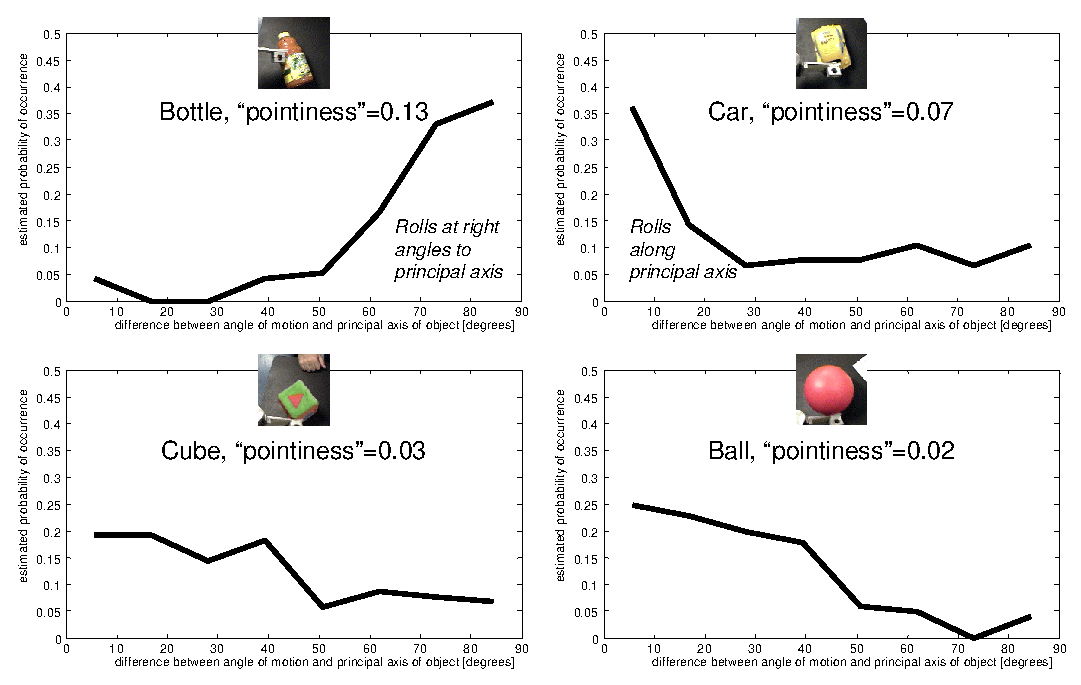
\includegraphics[width=\columnwidth]{affordances.eps}
\caption{ 
%
Probability of observing a roll along a particular direction for the set
of four objects used in our experiments. Abscissae represent the difference
between the principal axis of the object and the observed direction of 
movement. Ordinates the estimated probability.
%
}
\label{fig:affordances}
\end{center}
\end{figure}

This description of the affordances shows clear differences between the
objects.
But it is not yet an {\em effective} description since
it does not by itself tell the robot how to take
action once an object is observed. For this purpose a description of 
the geometry of poking is required.
%: i.e. the description of the properties of 
%objects (Figure \ref{fig:affordances}) has to be connected to a description
%of the behavior of the object. 
This information can be derived from the same training set we collected for learning
about rolling. Figure \ref{fig:actions} shows the histograms of the direction 
of movement averaged over all objects for
each possible action. For example, the back slap moves an object mostly upward
(about $-100^\circ$ on average, $0^\circ$ being the direction parallel to the image
$x$ axis) and away from the robot. A similar consideration applies
to the other poking gestures. Figure \ref{fig:actions} was obtained from the data of
about 500 poking events.

The last step is to connect all these elements together. If a known object is
presented to Cog, the object is recognized, localized, and
its orientation estimated (by finding its principal axis). Recognition is based on the color histograms. The same
procedure used to form the clusters is employed here. Localization is simply implemented 
by histogram back-projection and a search across the image. The current orientation of the
object is then estimated by comparing the current image with all the prototypes 
contained in the cluster. The whole procedure has an error on the estimation
of the principal axis in the range of $10^\circ$ to $25^\circ$ depending on the object.  

To actually exploit the understanding of the affordance we need to connect vision to 
behavior. The robot looks for the preferred rolling direction of the object
(see figure \ref{fig:affordances}) and adds it to its current orientation. 
The action whose effects are closer (on average) to the combination of the orientation
and affordance is selected.

% TEST OF PERFORMANCE MISSING?
We performed a simple qualitative test of the robot's behavior presenting randomly
two of the objects (the toy car and the bottle) - note that the ball and the cube 
do not have a well defined principal axis so there is no point in running the 
experiment. Out of 100 trials the robot made 15 mistakes. Analysis 
of the errors reveals that they are mainly due to imprecise control (12) and to a
less extent to misinterpretation of the orientation of the object (3).

\begin{figure}[tb]
\begin{center}
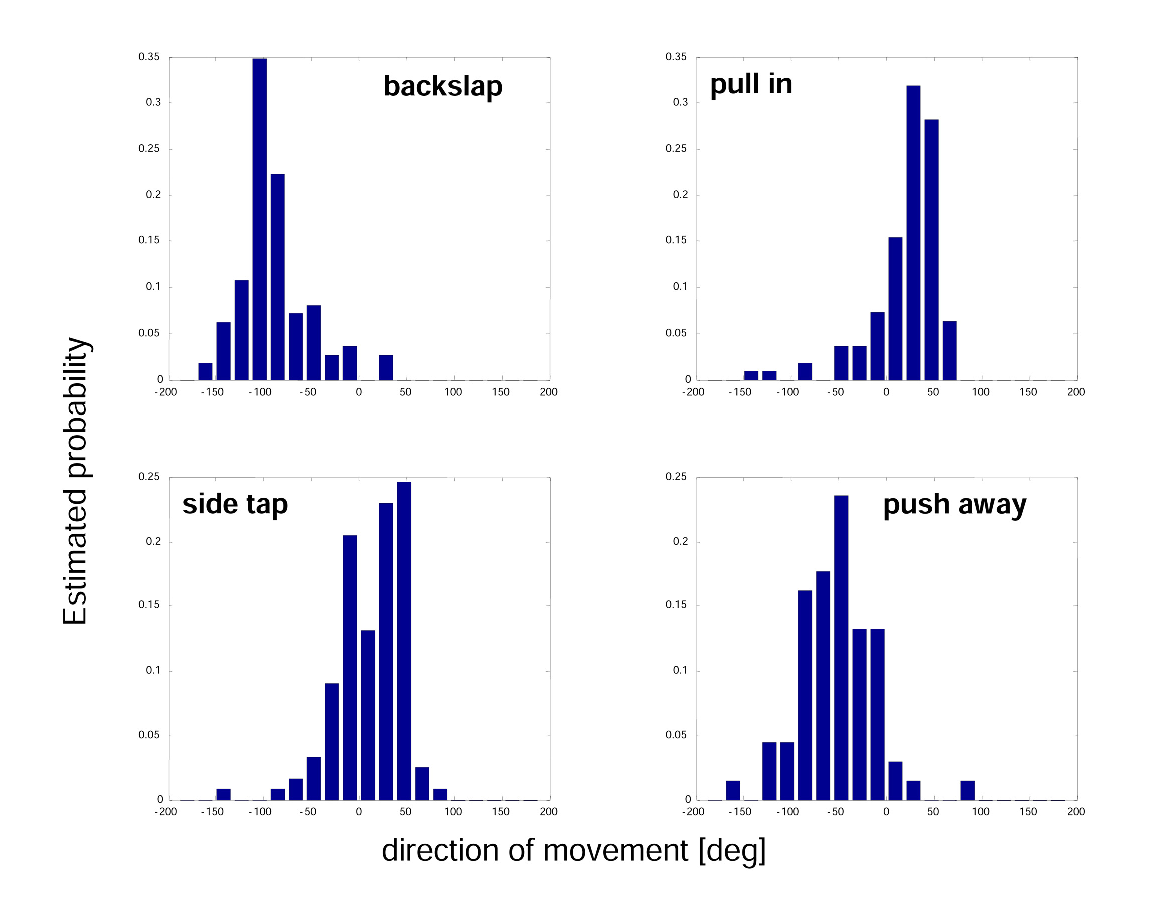
\includegraphics[width=12cm]{actions.eps}
\caption{ 
%
Histogram of the direction of movement of object for each possible poking action.
For each of the four plots the abscissa is the direction of motion of the object
where the $0^\circ$ direction is parallel to the x axis, and $-90^\circ$ to the y
axis. The ordinate is the empirical probability distribution of the direction
of motion of the objects.
%
}
\label{fig:actions}
\end{center}
\end{figure}


\section{Developing mirror neurons}
\label{sec:mirror}

\ifverbose
\begin{figure}[tb]
\begin{center}
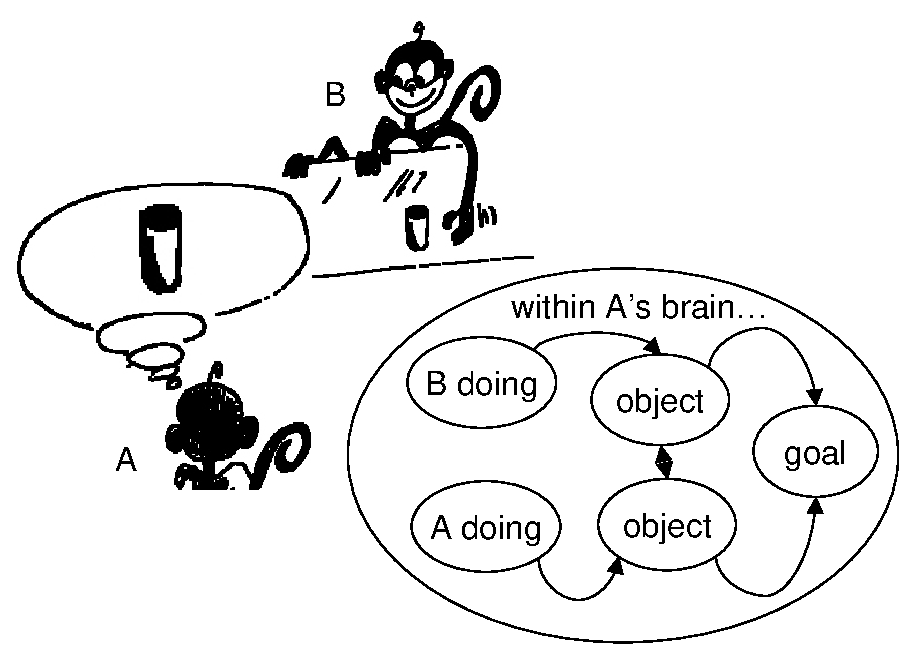
\includegraphics[width=\columnwidth]{mirror-monkey.eps}
\caption{ 
%
Mirror neurons and causality: from the observer's point
of view (A), understanding B's action means mapping it onto the
observer's own
motor repertoire. If the causal chain leading to the goal is already
in place (lower branch of the graph) then the acquisition of a
mirror neuron for this particular action/object is a matter of
building and linking the upper part of the chain to the lower one.
There are various opportunities to reinforce this link either at the object
level, at the goal level or both. 
%%Developmentally we can explain
%%mirror neurons only if we take into account another class of neurons
%%(called canonical) which in practice describes the lower branch of the
%%graph.
%
}
\label{fig:mirror-monkey}
\end{center}
\end{figure}
\fi

An interesting question then is
whether the system could extract useful information from seeing an
object manipulated by someone else.  In the case of poking, the robot
needs to be able to estimate the moment of contact and to track the arm
sufficiently well to distinguish it from the object being poked.  We
are interested in how the robot might learn to do this.  One approach
is to chain outwards from an object the robot has poked.  If someone
else moves the object, we can reverse the logic used in poking --
where the motion of the manipulator identified the object -- and
identify a foreign manipulator through its effect on the object.
The next experiment was designed to explore this aspect.

In fact, the same processing used for analyzing an active poking 
can be used to detect a contact and segment the object from the manipulator.
This is not different from what we used for learning. While one might argue then
that learning can be carried out just by mere observation, it is
worth noting that: i) this situation is not as well defined  
as the active one, and ii) there is no connection to the motor aspects 
of the action and consequently it is difficult to link the observation to the behavior.
There is no physical contact, thus there is plenty of room for getting confused 
by false positives. The temporal aspect, so well constrained during active manipulation, is 
more vague here -- the robot, for example, does not know when the foreign manipulator starts
or stops the action. If missing a contact event or getting a false or mistaken 
segmentation is not much of a problem in ``observation mode'', it is much more
troublesome is we corrupt the training data with unreliable/noisy observations.
Further, we should not assume the human ``teacher'' is truly collaborative. 
There is no guarantee that actions suited to the robot perceptual system and/or 
goal are performed at all.
More seriously, the link to behavior is completely missing. Even if visual 
information about objects can be collected as before, tracing back which action
causes a particular consequence cannot be autonomously learned by the robot.
Conversely, in the case the robot has already learned about objects, 
as e.g. we have shown in the previous section, this information can be
factored in to help the observation of somebody else's action. Touch 
(not in Cog) and physical contact are additional bits of information 
about the ongoing activity.

In our case, if any activity is detected close to the object -- measured by the 
amount of motion in a neighborhood of the fixation point corresponding to the robot's foveal 
camera -- reaching is inhibited and the whole action observed (assuming there 
is one at all). An example of human poking is shown in figure \ref{fig:observed-action}.

\begin{figure}[tb]
\begin{center}
%%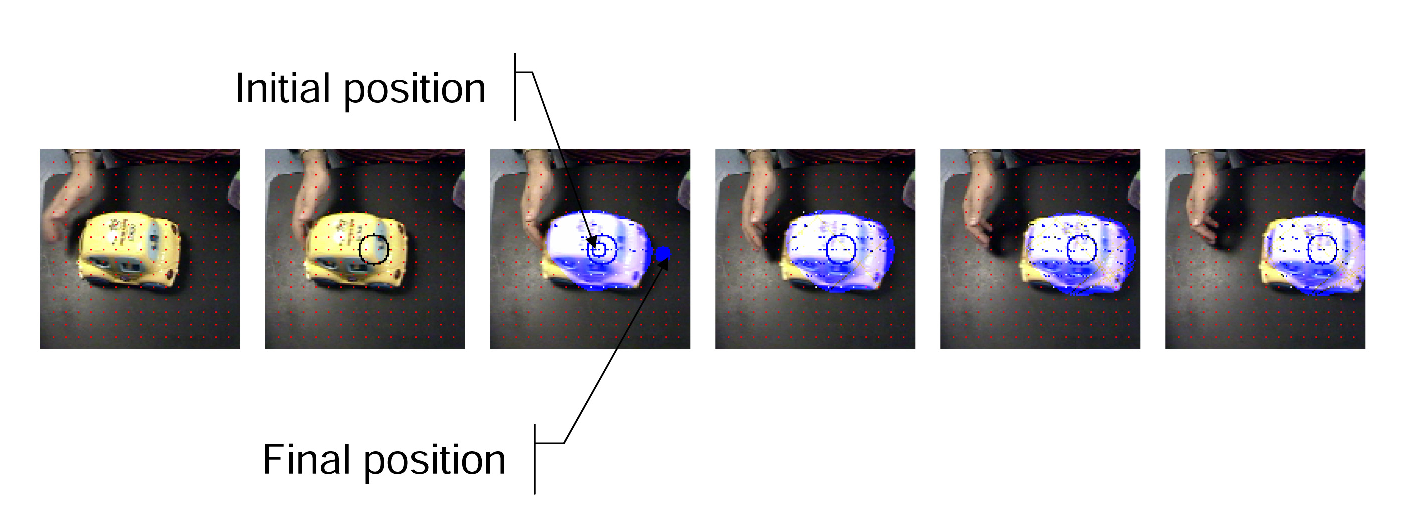
\includegraphics[width=\columnwidth]{observed-action.eps}
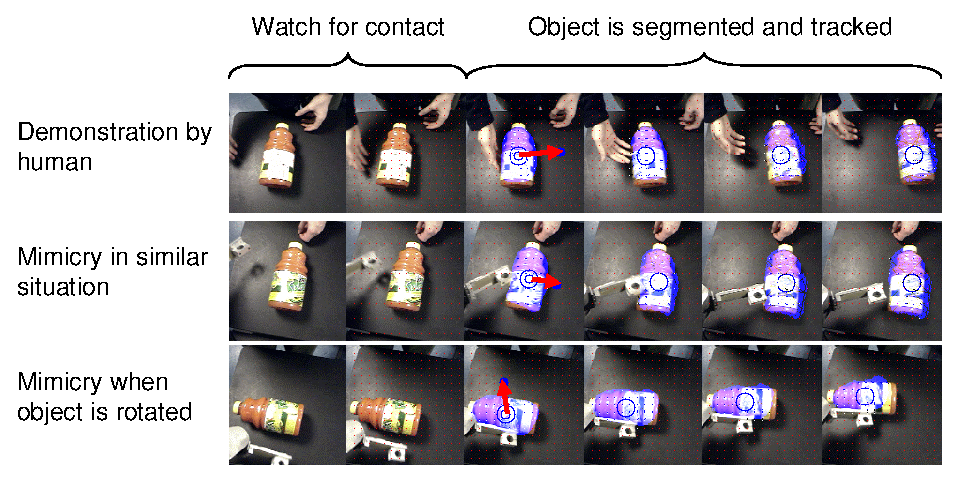
\includegraphics[width=\textwidth]{fig-mimicry-bottle}
\caption{ 
%
Basic mimicry.  The first step in mimicking an action is to actually
be able to observe it.  The first sequence shows a human demonstration
of a poking operation.  Frames around the moment of contact are shown.
The object, after segmentation, is tracked for 12 frames using a
combination of template matching and optic flow.  The big circles
represent the tracked position of the bottle in successive frames.
The arrow displayed on the frame of contact ($3^{rd}$ from the left)
projects from the position at the time of contact and at the $12^{th}$
frame respectively.
%
In the second sequence, the bottle is presented to the robot in the
same orientation it had in the demonstrated action and the robot
repeats the observed action, a ``side tap''.  In the third sequence,
the car is presented at a different angle.  The appropriate action to
exploit the affordance and make the bottle roll is now a ``back
slap''.
%
%An example of observed sequence with tracking superimposed. 
%Frames around the
%moment of contact are shown. The object, after segmentation, is tracked for 12 
%frames using a combination of template matching and optic flow. The big circles
%represent the position of the toy car in successive frames. The two small circles
%(outline and solid) displayed on the frame of contact ($3^{rd}$ from the left) are 
%the position at the time of contact and at the $12^{th}$ frame respectively.
%
}
\label{fig:observed-action}
\end{center}
\end{figure}

The first obvious thing the robot can do is to identify the action just observed 
with respect to its motor vocabulary. It is easily done, in this case, by comparing 
the displacement of the object with the four possible actions and by choosing the
action whose effects are closer to the observed displacement.
Indeed it allows -- even if in this limited setting -- recognizing 
a complex action by interpreting its consequences on the environment.
This is orders of magnitude simpler than trying to completely characterize the
action in terms of the observed kinematics of the movement. Here, the complexity
of the data we need to obtain from the observations is somehow proportional to the complexity
of the goal rather than that of the structure/skills of the foreign manipulator. In our case, because 
the action, the goal, and the object are relatively simple, the only information 
required is about the displacement of the object. 

Therefore, the next question is whether we can use this ``understanding'' of 
observed actions to implement mimicry behavior. It 
would be easy now to try to replicate the action just observed if the same
object were presented again. However, there is still a bit of ambiguity in that
we can choose to mimic either the observed displacement of the object or 
the way the object was poked with respect to its rolling affordance.
 
We chose to implement the latter. It is clear that poking along a particular 
observed direction requires trivial modifications. In practice, after an 
action is observed the angle between the affordance (see table \ref{tab:affordances}) and
the actual displacement is measured and stored. If it happens to see the same 
object again, the robot chooses the action that has the greatest 
probability of poking the object along the previously stored angle. 
Figures \ref{fig:observed-action} and \ref{fig:mimicked-action} show examples of such mimicry.
%Figure \ref{fig:mimicked-action} shows two examples of mimicry as a consequence of the
%action shown in figure \ref{fig:observed-action}.

\begin{figure}[tb]
\begin{center}
%%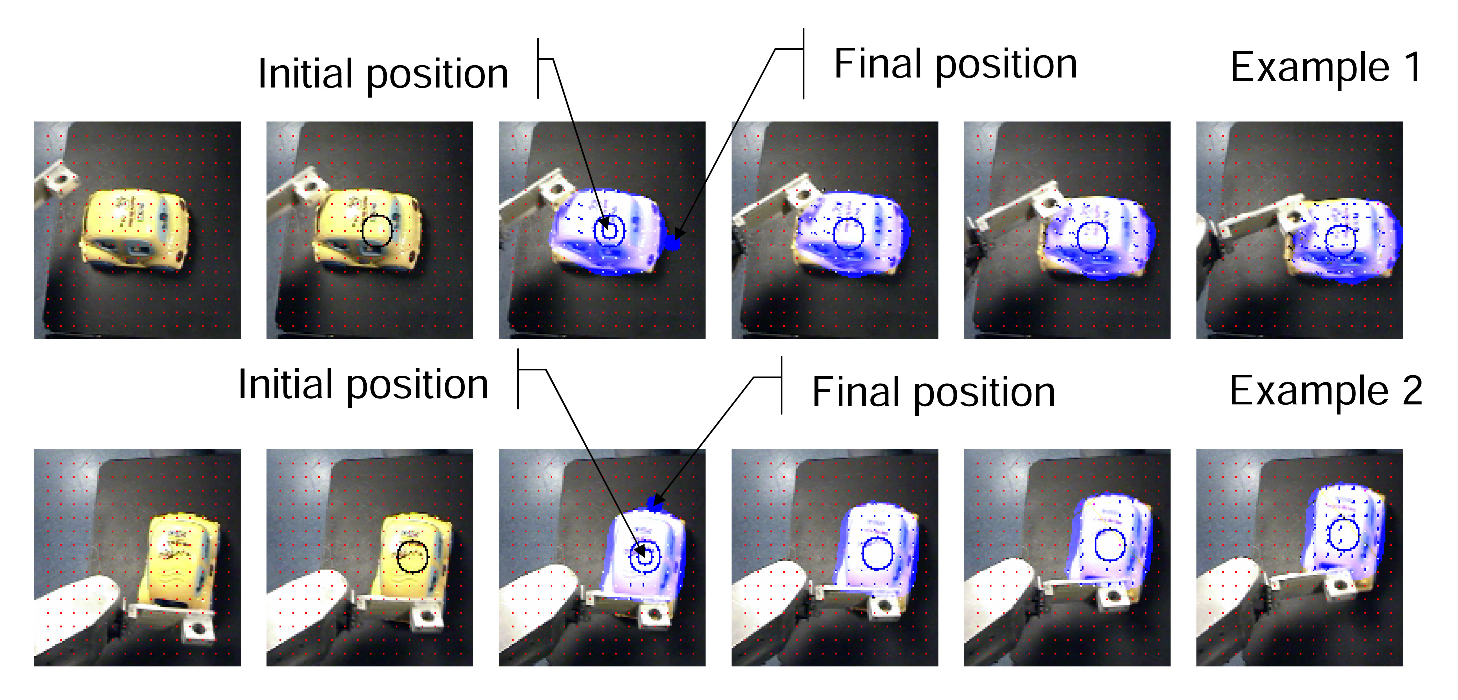
\includegraphics[width=\columnwidth]{mimicked-action.eps}
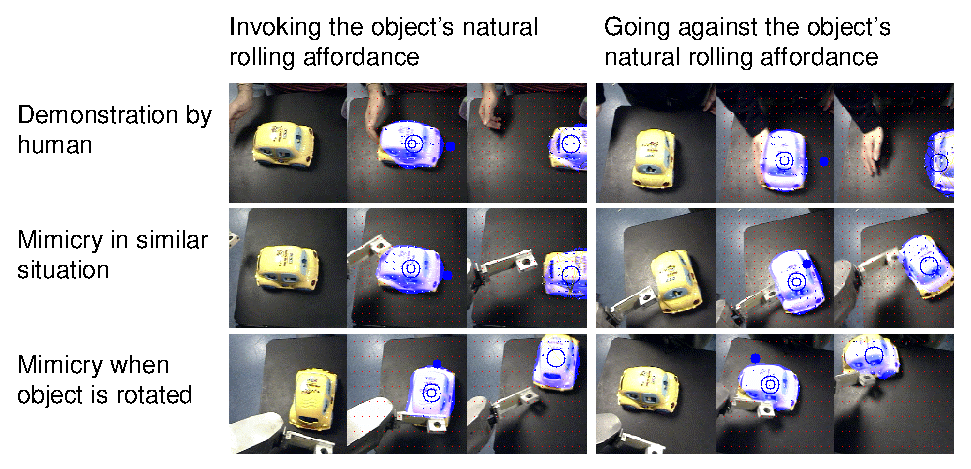
\includegraphics[width=\textwidth]{fig-mimicry-awkward.eps}
\caption{ 
%
An extended mimicry example using the toy car.
The sequences on the left show the robot mimicking a human exploiting
the car's rolling affordance.  The sequences on the right show
what happens when the human hits the car in a contrary fashion, going
against its preferred direction of motion.  The robot mimics this 
``unnatural'' action, suppressing its usual behavior of trying to
evoke rolling.
%OUTDATED Two examples of mimicry following the observation in figure \ref{fig:observed-action} 
%where a human manipulator pokes the toy car exploiting the affordance (the car rolls). 
%In example 1 (top row), the toy car has the same orientation it had in the
%demonstrated action and the robot repeats the observed action. In example 2 (bottom), 
%the car is $90^\circ$ with respect to example 1. The appropriate action to exploit
%the affordance and make the car roll is thus a back slap. 
%
}
\label{fig:mimicked-action}
\end{center}
\end{figure}

This response is exactly what we would expect from a ``mirror-type'' representation.
The observed action is interpreted on the basis of the robot own motor code. The same
data structure is also used/activated when performing an action in response to the
sight of a known object. The causal link between the two events that could be separated
by several seconds is the object, the goal, and the object's affordances. There is 
considerable precedent in the literature for a strong connection between viewing 
object manipulation performed by either oneself or another \cite{wohlsclager02human}.
There is also a growing evidence that imitation is goal-directed 
\cite{bekkering-wohlschlager-2000} and that the object of the action is explicitly 
coded (e.g. during reaching) \cite{woodward-1998}.


\ifverbose
Poking is an ideal testbed for future work on this, since it is much
simpler than full-blown object manipulation and would only require a
very simple model of the foreign manipulator to work.

There is considerable precedent in the literature for a strong
connection between viewing object manipulation performed by either
oneself or another \cite{wohlsclager02human}.  As we already mentioned
F5 contains a class of neurons called canonical neurons that have a
very specific response when an object is being either manipulated or
fixated.  Grossly simplifying, we might think of canonical neurons as
an association table of grasp/manipulation (action) types with object
(vision) types.  Another class of neurons called ``mirror neurons''
can then be thought of as a second-level association map which links
together the observation of a manipulative action performed by
somebody else with the neural representation of one's own action.

Figure~\ref{fig:mirror-monkey} shows this causal chain in action.
There are a series of interesting behaviors that can be realized based
on mirror neurons. Mimicry is an obvious application, since it
requires just this type of mapping between other and self in terms of
motor actions.  Another important application is the prediction of
future behavior from current actions, or even inverting the causal
relation to find the action that most likely will get to the desired
consequence.
\fi

\ifverbose

for example, by observing the part of an action the robot or the
bioagent can come out with suitable expectations of the consequences
of that action. On the other hand, the inverse behavior can also be
foreseen. The latter account to inverting the causal relation and
getting the action that most likely will get to the desired
consequence.

It might be argued that we need a two stages procedure to learn a
mirror representation, where we first learn ``something'' and only
subsequently we ``understand'' other people's behavior. The actual
developmental course might not be such artificially staged. A slight
advantage must be given though to the initial step of self-learning,
the understanding comes later.


This set of associations can be learned autonomously (by a robot for
example) simply by a trial and error procedure and possibly with a
reinforcing signal to tell when a given grasp/manipulatory gesture was
successful if applied to a particular object.

We should not probably think of this association as describing in
detail the object being manipulated visually. Perhaps only features
relevant to manipulation are stored (e.g. size, orientation in space).
This representation is a ``pragmatic'' one describing only those
properties of objects are needed to apply a particular set of actions
to them. Affordances are a good psychological analogue of F5
canonical neurons.
\fi


\ifverbose
How does this relate to causation?  The two situations in some sense
share the same goal, and more practically share the same object.  The
whole procedure assumes a basic discrimination of size and shape of
objects (not necessarily categorization in traditional sense), and the
exploitation of the visual information to the understanding of the
grasp type. In some cases though the goal might be unambiguous, e.g. a
needle is very unlikely grasped with a full palm grasp, as well as a
box is not grasped with a pinch grip. These are the most informative
allowing for the best discrimination of action type from the visual
perspective.
\fi

\ifverbose
The definition of imitation we gave here implicitly focus on imitating
the goal rather than the precise trajectory. This automatically takes
into account any difference in body structure between the actor and
the observer.

Of course, manipulation as in poking can lead to a better
understanding of the physical properties of objects not directly
amenable to visual exploration such as mass, roughness, softness, etc.
\fi


\section{Towards object recognition}

\label{sect:recognition}

\begin{figure}[tbh]
\begin{center}
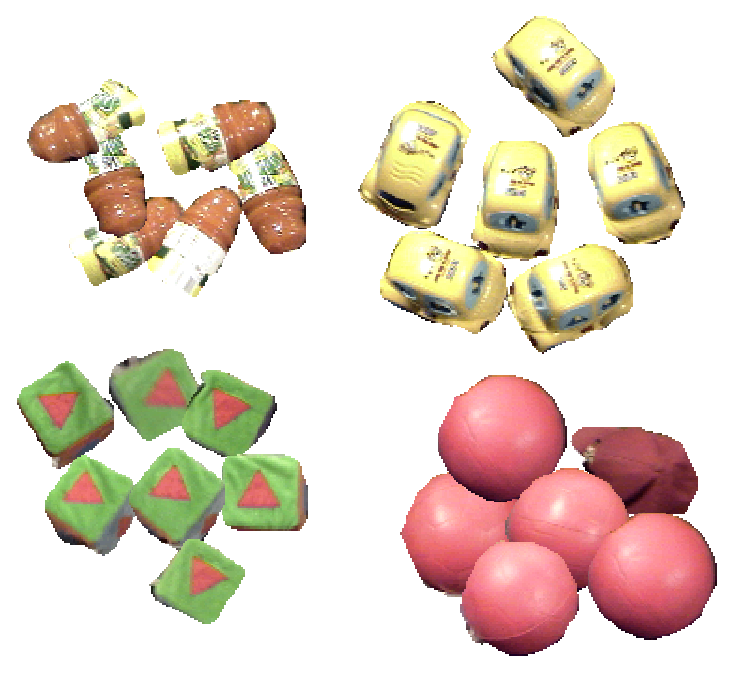
\includegraphics[width=10cm]{fig-object-clusters2.eps}
\caption{ 
%
Once objects have been segmented from the background, they are much
easier to distinguish from each other since the irrelevant similarity
of their shared environment is eliminated.  To build object models,
the robot clusters all the segmented views it receives based on
similarity of their color histogram.  This figure shows samples from
four of the clusters found, corresponding to the four objects used in
Section~\ref{sect:experiment}.  Note the baseball cap classified with
the ball, lower right -- a young child wandered by the robot while we
were collecting data and got it to poke his cap.
%
}
\label{fig:objects-clusters}
\end{center}
\end{figure}

Although poking is a very crude and primitive form of manipulation we have
shown that it can help to bootstrap more complex behaviors without relying on 
an external teacher. With only minimal assumptions (using motion as segmentation
cue) we were able to build a system that exploits its environment to 
learn novel behaviors. If Cog had a dextrous hand, it could further
exploit temporal constraints (e.g. an object remains the same unless it is dropped)
to collect tightly/temporally correlated data. 
\ifrev
There are already examples in robotics of the acquisition of
object categorization based on this kind of temporally correlated information 
\cite{scheier-lambrinos-1996}.
\fi
This form of ``object constancy'' could be 
exploited for instance to learn about an object with confusing visual features such
as many different colors, different geometric patterns, and so forth  
(see the example of the cube in figure \ref{fig:sample-results}). A finer form of manipulation can be
used also to group objects on the basis of their behavior rather than purely
by visual appearance: e.g. the class of ``bottle'' or of ``toy cars''.
This, in some future implementation, can help the robot to attain a goal by using
a suitable tool (among many) rather than exactly the same tool it used
when initially learned the task.

A possible and obvious extension is to use the object segmentation provided 
by poking (and manipulation in general) to build models of the appearance of objects 
beyond the color histogram we used in our experiments (think again about the
colored cube shown in figure \ref{fig:sample-results}).
Also in this case the robot could work autonomously on learning. Furthermore, the
interaction between manipulator and object provides another element that can
be used to learn about the manipulator itself (see figure \ref{fig:manipulator}). 
The robot can then learn about the appearance of its own hand or, 
equally, about the human hand. It is remarkable that the complexity of 
the robot manipulator does not necessarily have to match that of the human 
manipulator. We can envision a similar procedure to learn about any object that 
functions as manipulator.
%
%
%
%We can envision a similar procedure to learn about 
%any object that functions as manipulator.
%

\begin{figure}[tb]
  \centerline{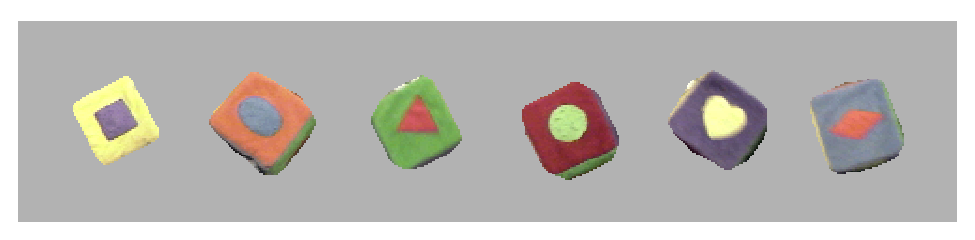
\includegraphics[width=9cm]{fig-cube-segmentations}}
%%  \centerline{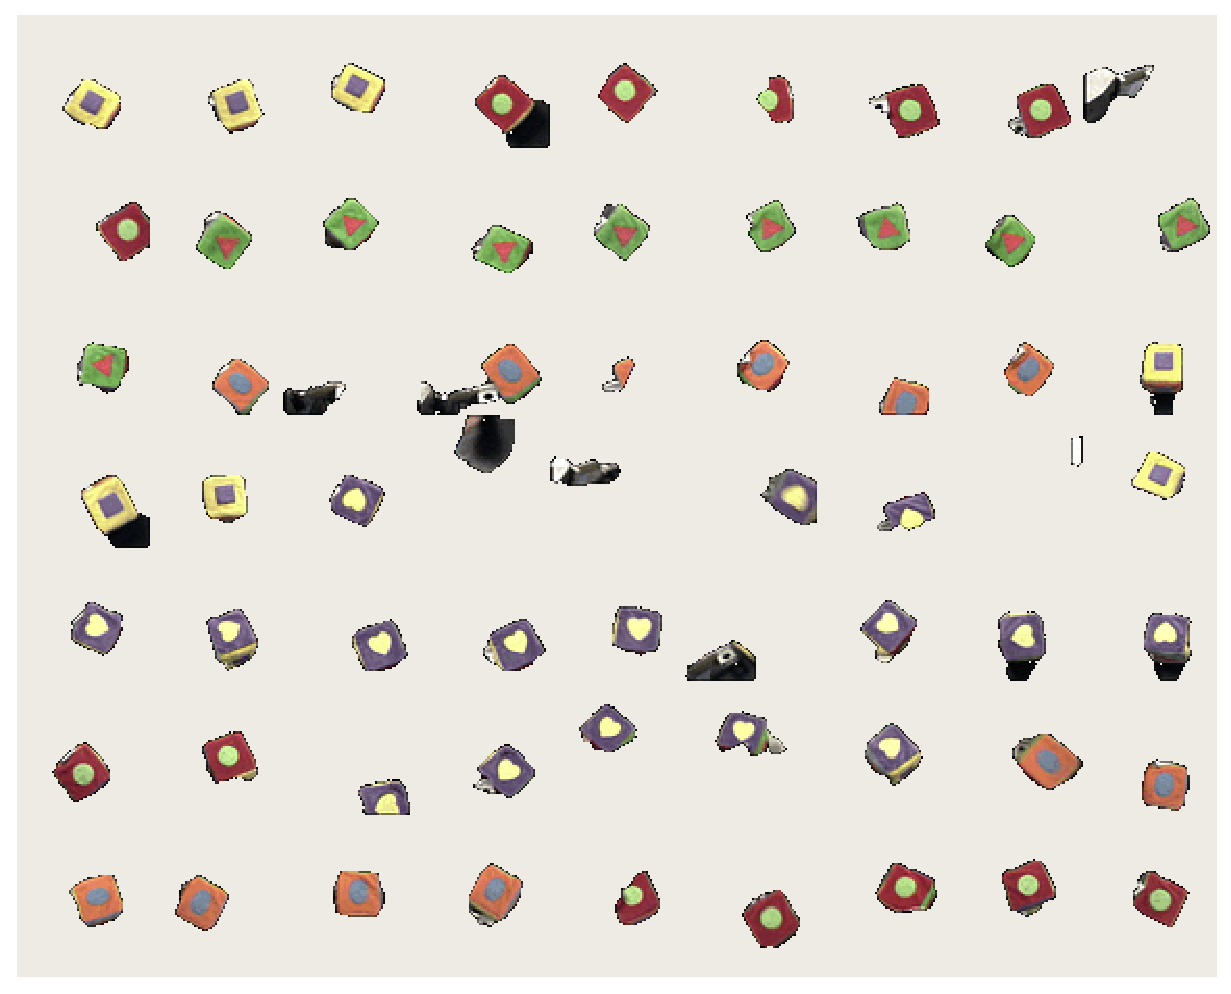
\includegraphics[width=9cm]{experiment-montage}}
  \caption{
%
Poking also gives the robot the opportunity
to collect many views of a single object, and so we can hope to deal
with recognizing objects like this toy cube
that has a different appearance from every side (the segmentations
shown here were collected automatically).
%
}
  \label{fig:sample-results}
\end{figure}





\section{Learning about manipulators}

How could a robot find human arms and hands in the environment without
any prior knowledge of their appearance?  We could imagine segmenting
any moving objects in the scene, and relying on the heuristic that
hands are often the fastest moving objects around [cite].
Another approach is possible in our situation.  If the robot can
detect when an impact event occurs, it can collect segmentations of the
object that caused the impact.  The set of objects that habitually
trigger the motion of other objects is not a bad operational 
definition of a manipulator, and should include the human hand/arm,
and the robot's own arm.

Unconstrained motion in a scene is difficult to parse.  But since the
robot has become familiar with a set of objects through poking, it can
constrain the scenarios in which it may identify the manipulator.  In
particular, fixating a familiar object is a necessary condition for
reliably detecting collision.  Fixation is improved by object recognition
and localization, trained my the previous poking episodes.

May fail for more complex events -- e.g. other motion, shadows cast on
object etc.

When the robot fixates an object that it can reach, it will try to poke it.
This is inhibited if it sees motion around the object, giving a human the
opportunity to poke it instead.

The point of contact detection will still work in this case, since it 
doesn't rely on the manipulator being the robot's own arm.

The frames leading up to the impact are great for detecting the
appearance of the manipulator itself.  And give a strong cue that the
moving object is in fact a manipulator (something used to impact
objects).  See Figure~\ref{fig:manipulator}.

\begin{figure}[tbh]
  \centerline{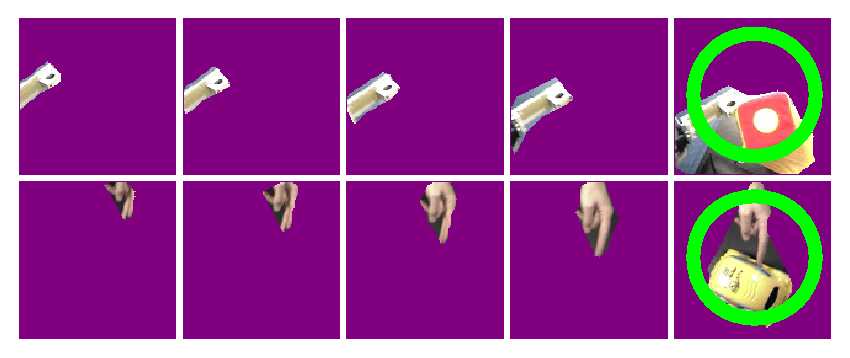
\includegraphics[width=\textwidth]{manipulator-segment}}
  \caption{Early experiments on segmenting the robot arm, or a 
human hand poking an object the robot is familiar with, by working
backwards from a collision event.}
  \label{fig:manipulator}
\end{figure}

Can't necessarily remove shadow.



